\documentclass[10pt]{exam}

\usepackage[margin=1in]{geometry}
\usepackage{amsmath}
\usepackage{amssymb}
\usepackage{amsthm}
\usepackage{mathtools}
\usepackage{bm}

\usepackage{color}
\usepackage{colortbl}
\definecolor{deepblue}{rgb}{0,0,0.5}
\definecolor{deepred}{rgb}{0.6,0,0}
\definecolor{deepgreen}{rgb}{0,0.5,0}
\definecolor{gray}{rgb}{0.7,0.7,0.7}

\usepackage{hyperref}
\hypersetup{
  colorlinks   = true, %Colours links instead of ugly boxes
  urlcolor     = black, %Colour for external hyperlinks
  linkcolor    = blue, %Colour of internal links
  citecolor    = blue  %Colour of citations
}

%%%%%%%%%%%%%%%%%%%%%%%%%%%%%%%%%%%%%%%%%%%%%%%%%%%%%%%%%%%%%%%%%%%%%%%%%%%%%%%%

\theoremstyle{definition}
\newtheorem{problem}{Problem}
\newtheorem{defn}{Definition}
\newtheorem{refr}{References}
\newtheorem{theorem}{Theorem}
\newcommand{\E}{\mathbb E}
\newcommand{\R}{\mathbb R}
\DeclareMathOperator{\nnz}{nnz}
\DeclareMathOperator{\determinant}{det}
\DeclareMathOperator{\Var}{Var}
\DeclareMathOperator{\rank}{rank}
\DeclareMathOperator{\prob}{\mathbb P}
\DeclareMathOperator*{\argmin}{arg\,min}
\DeclareMathOperator*{\argmax}{arg\,max}

\newcommand{\Ein}{E_{\text{in}}}
\newcommand{\Eout}{E_{\text{out}}}
\newcommand{\Etest}{E_{\text{test}}}
\newcommand{\I}{\mathbf I}
\newcommand{\Q}{\mathbf Q}
\newcommand{\p}{\mathbf P}
\newcommand{\pb}{\bar {\p}}
\newcommand{\pbb}{\bar {\pb}}
\newcommand{\pr}{\bm \pi}

\newcommand{\trans}[1]{{#1}^{T}}
\newcommand{\loss}{\ell}
\newcommand{\w}{\mathbf w}
\newcommand{\wstar}{{\w}^{*}}
\newcommand{\x}{\mathbf x}
\newcommand{\y}{\mathbf y}
\newcommand{\lone}[1]{{\lVert {#1} \rVert}_1}
\newcommand{\ltwo}[1]{{\lVert {#1} \rVert}_2}
\newcommand{\lp}[1]{{\lVert {#1} \rVert}_p}
\newcommand{\linf}[1]{{\lVert {#1} \rVert}_\infty}
\newcommand{\lF}[1]{{\lVert {#1} \rVert}_F}

\newcommand{\ignore}[1]{}

%%%%%%%%%%%%%%%%%%%%%%%%%%%%%%%%%%%%%%%%%%%%%%%%%%%%%%%%%%%%%%%%%%%%%%%%%%%%%%%%

\begin{document}


\begin{center}
{
\Huge
Chapter 1: The Learning Problem (II)
}
\end{center}

\begin{center}
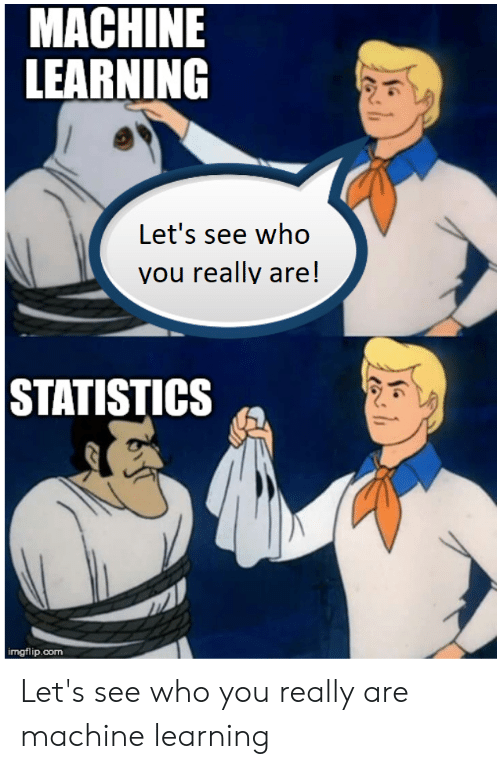
\includegraphics[height=3in]{scooby}
~~~~~~~~~~
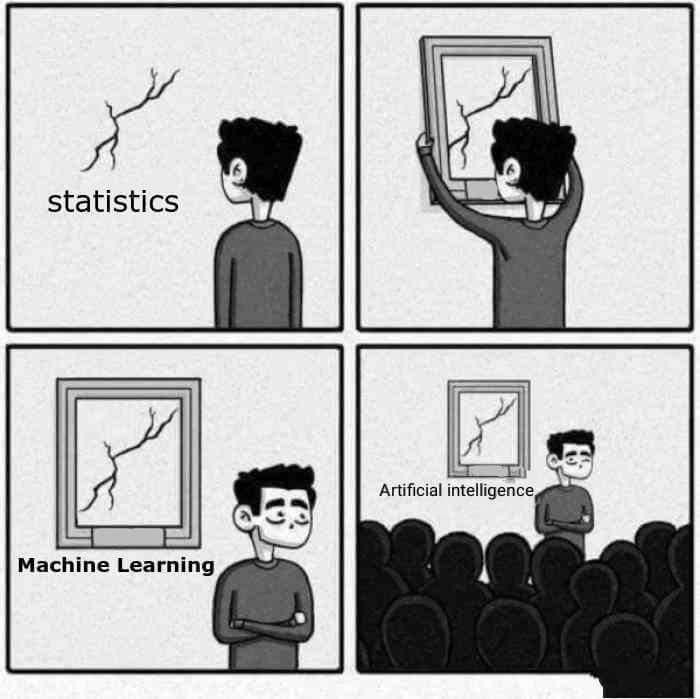
\includegraphics[height=3in]{ml}
\end{center}

\section{Section 1.1.3: Learning vs Design}

\begin{problem}
You should complete Exercise 1.5 to get practice identifying when to use a learning approach to a problem, and when to use a ``design'' approach to a problem.
\end{problem}

%\section{Section 1.2: Types of Learning}
%
%The textbook identifies 3 types of learning: supervised, reinforcement, and unsupervised.
%Pagerank is an example of an unsupervised algorithm (because we do not have ``labels'' about which nodes in the graph are the most important).
%The focus of the rest of this class will be on supervised methods.
%
%\begin{problem}
    %You need to be able to identify examples of the different learning types.
    %Exercise 1.6 will give you practice with this.
%\end{problem}

\newpage
\section{Section 1.3: Is Learning Feasible? and \\ Section 1.4: Error and Noise}

\begin{problem}
    Draw Figure 1.11, highlighting the differences between Figure 1.9 and Figure 1.2.
\end{problem}

%\begin{problem}
    %When our dataset , it is impossible to ``guarantee'' that we get the correct solution when training.
    %Read Section 1.3.1 and complete Exercise 1.7 to see an example problem 
%\end{problem}

\newpage
\begin{problem}
    In this problem we will explore the train/test split protocol for training machine learning algorithms.
    \begin{enumerate}
        \item Define the in-sample error and out-of-sample errors (page 21).
            \vspace{3in}
        \item A fundamental goal of the machine learning discipline is to understand the out-of-sample error of different algorithms.
            One of the most powerful tools for doing this is Hoeffding's inequality.
            It is introduced informally in the textbook on page 19, Eq (1.4) in the context of a toy example involving marbles.
            The following formally stated theorem is a bit more versatile, and it's what we'll rely on in this class.
            \begin{theorem}[Hoeffding Inequality]
                Let $a_1, ..., a_N$ be $N$ independent and identically distributed random variables satisfying $0 \le a_i \le 1$.
                Let $\nu = \tfrac1n\sum_{i=1}^N a_i$ be the empirical average and $\mu = \E \nu$ be the true mean of the underlying distribution.
                Then, for all $\epsilon > 0$,
                \begin{equation}
                    \label{eq:hoef}
                    %\prob\big(|S_n - \E[S_n]| \ge t\big)
                    \prob\big(|\nu - \mu| \ge \epsilon\big)
                    \le 
                    2 \exp (-2\epsilon^2 N)
                    .
                \end{equation}
            \end{theorem}
            Describe the shape of the distribution defined by inequality \ref{eq:hoef} above.

        \newpage
        \item Let $g$ be the output of running the PLA on the training data.
            What does Hoeffding's inequality say about the out-of-sample error?
            \vspace{6in}

        %\item Why is the Hoeffding inequality an example of a PAC learning bound?
            %\vspace{4in}

        %\item You want to ``guarantee'' that the test error $\Etest$ is a good approximation of the true error $\Eout$.
            %Of course, you can't guarantee this, you can only make it ``probably'' true.
    \end{enumerate}
\end{problem}
\newpage
\begin{problem}
    How large of a test set do you need to guarantee with probability at least 0.99 that $|\Etest-\Eout| \le 0.01$?
\end{problem}

\newpage
\begin{problem}
    This problem explores the optimal way to size your test sets.
    \begin{enumerate}
        \item If you have a test set with 1000 samples, what bound does the Hoeffding inequality give on the probability that $|\Etest-\Eout| \le 0.01$?
            \vspace{1.5in}

        \item
            Why is this bound ``trivial''?
            \vspace{1.5in}

        \item
            What if you change the accuracy to $|\Etest-\Eout| \le 0.05$?
            \vspace{1.5in}

        \item
            What if you use the original accuracy $|\Etest-\Eout| \le 0.01$ but use 10000 samples in your test set?
            \vspace{1.5in}

        \item
            If we expect the accuracy of our learning algorithm to be close to 1 (i.e.\ we expect $|\Etest-\Eout|$ to be close to 0),
            should we use a larger or a smaller test set than when we expect the accuracy to be close to 0.8 (i.e.\ we expect $\Etest-\Eout|$ to be close to 0.2)?
            \vspace{1.5in}
    \end{enumerate}
\end{problem}

\ignore{
\begin{problem}
    The goal of PAC learning bounds is to help us choose which model to use for a particular problem.
    (Recall that a model is a hypothesis class plus a learning algorithm.)
    In this problem, we will explore some simple, finite hypothesis classes.
\end{problem}

\begin{theorem}[Union Bound]
    For any set of events $\mathcal B_1, ..., \mathcal B_n$,
    we have that
    \begin{equation}
        \prob\left(\bigcup_{i=1}^n \mathcal B_i\right)
        \le
        \sum_{i=1}^n \prob(\mathcal B_i)
        .
    \end{equation}
\end{theorem}

%\begin{problem}
    %Define the
    %\begin{enumerate}
        %%\item Hoeffding Inequality (page 19, Eq 1.4)
        %%\item in-sample error (page 21)
        %%\item out-of-sample error (page 21)
        %\item Eq 1.5
        %\item union bound (page 24)
        %\item Eq 1.6
    %\end{enumerate}
%\end{problem}

\begin{problem}
    In practice, computers implement IEEE754 floating point arrithmetic rather than real number arithematic.
    This means that all hypothesis classes (that are used in practice) are actually finite.
\end{problem}

\begin{problem}
    Complete Exercise 1.11.
\end{problem}

\begin{problem}
    Complete Exercise 1.12.
\end{problem}

%\section{Section 1.4: Error and Noise}
%
\begin{problem}
    Complete Exercise 1.13
\end{problem}

\begin{problem}
    For each statement below, indicate whether the claim is True, False, or Open.
    \begin{enumerate}
        \item More complicated models need a larger training set to deterime
    \end{enumerate}
\end{problem}

}

\end{document}



